\PassOptionsToPackage{unicode}{hyperref}
\documentclass[aspectratio=1610, 9pt]{beamer}

\usetheme{vertex}

\newfontfamily\zigarette{TeX Gyre Heros}

\usepackage[main=ngerman, english]{babel}

\usepackage[autostyle]{csquotes}
\renewcommand{\mkblockquote}[4]{foo#1#2\par\hfill\footnotesize#4#3}

\usepackage[firstinits=true, style=authortitle]{biblatex}
\addbibresource{references.bib}
\DefineBibliographyStrings{german}{andothers = {{et\,al\adddot}}}  % replace u.a. with et al.

\usepackage{tcolorbox}

\usepackage{siunitx}

\usepackage{grffile}
\usepackage{graphicx}
\usepackage{tikz}
\usetikzlibrary{calc}
\tikzset{
  invisible/.style={opacity=0,text opacity=0},
  visible on/.style={alt={#1{}{invisible}}},
  alt/.code args={<#1>#2#3}{%
    \alt<#1>{\pgfkeysalso{#2}}{\pgfkeysalso{#3}} % \pgfkeysalso doesn't change the path
  },
}

\usepackage{hyperref}
\usepackage{bookmark}


\title{Farbwahrnehmung und Datenvisualisierung}
\author[maxnoe]{Maximilian Nöthe}
\date[SoAk19]{PeP et al. Sommerakademie 2019}
\institute{PeP et Al.}

\begin{document}
\maketitle

\begin{frame}[t]{Überblick}
  \tableofcontents
\end{frame}

\section{Menschliche Farbwahrnehmung}
\bumper{Menschliche Farbwahrnehmung}

\begin{frame}[c]{Geschichte}
  \begin{columns}[onlytextwidth]
    \hfill
    \begin{column}{0.59\textwidth}
      \begin{itemize}
        \item Erste physiologische Versuche durch Johann Wolfgang von Goethe (Zur Farbenlehre, 1810) \\
        \item Dreifarbentheorie (Young \& v. Helmholtz, 1804 / 1850)
        \item Gegenfarbtheorie (Ewald Hering 1878) \\
          \begin{tabular}{r @{${}⟷  {}$} l}
            blau & gelb \\
            rot & grün \\
            hell & dunkel \\
          \end{tabular}
        \item Erster Nachweis der Zapfen (Svaetichin, 1956) 
      \end{itemize}
    \end{column}
    \hfill%
    \begin{column}{0.39\textwidth}
      \hfill%
      \vfill%
      \centering
      \only<1>{%
        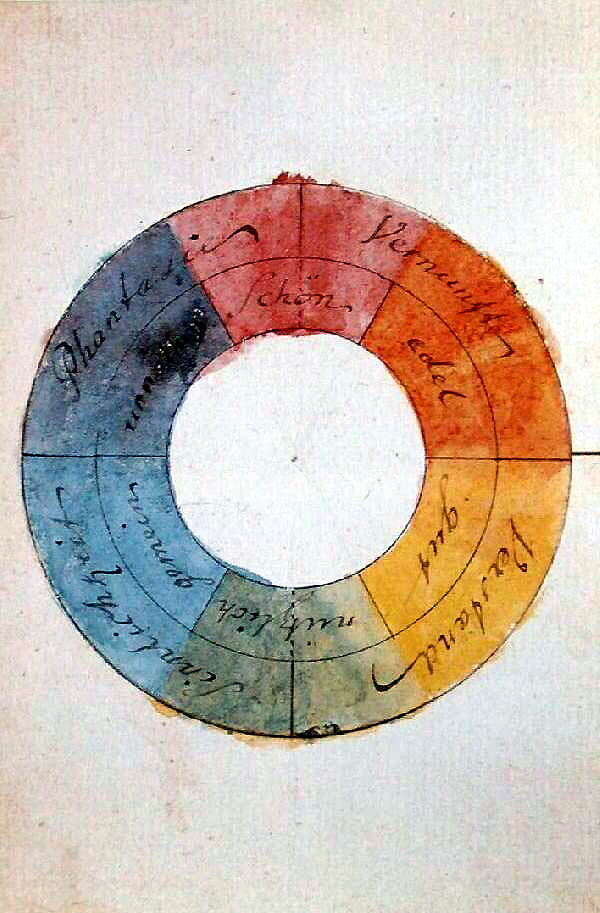
\includegraphics[width=\linewidth, height=0.90\textheight, keepaspectratio]{images/goethe_farbenkreis.jpg}

        [Goethe, 1809]
      }%
      \only<2>{%
        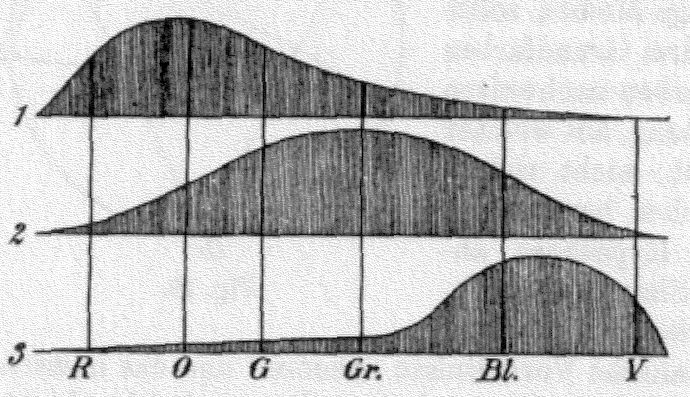
\includegraphics[width=\linewidth]{images/YoungHelm.jpg}

        [v. Helmholtz, 1894]
      }%
      \vfill%
    \end{column}%
  \end{columns}%
\end{frame}

\begin{frame}[c, plain]
  \centering
  \begin{tikzpicture}[shift=(current page.center), remember picture, overlay]
    \fill[color=green] (0, 0) rectangle (-0.2\textwidth, 0.2\textwidth);
    \fill[color=yellow] (0, 0) rectangle (0.2\textwidth, 0.2\textwidth);
    \fill[color=blue] (0, 0) rectangle (-0.2\textwidth, -0.2\textwidth);
    \fill[color=red] (0, 0) rectangle (0.2\textwidth, -0.2\textwidth);
    \fill[color=black] (0, 0) circle (0.02\textwidth);
  \end{tikzpicture}
\end{frame}

\begin{frame}[c, plain]
  \begin{tikzpicture}[remember picture, overlay, shift=(current page.center)]
    \fill[color=black] (0, 0) circle (0.02\textwidth);
  \end{tikzpicture}
\end{frame}


\begin{frame}[t]{Zapfen}
  \includegraphics{build/plots/cone_response.pdf} 
\end{frame}

\begin{frame}[t]{Zapfen}
  \includegraphics{build/plots/photopic.pdf} 
\end{frame}

\begin{frame}[t]{Farbfehlsichtigkeit}
  \begin{center}
    \includegraphics{build/plots/colorblind_response.pdf}
  \end{center}
  
  Prozentzahlen für weiße Männer. \\
  Wird X-chromosonal vererbt ${}⇒{}$ Frauen ca. quadratisch weniger
\end{frame}

\begin{frame}[t]{Farbfehlsichtigkeit}
  \begin{columns}[onlytextwidth]%
    \begin{column}{0.495\textwidth}%
      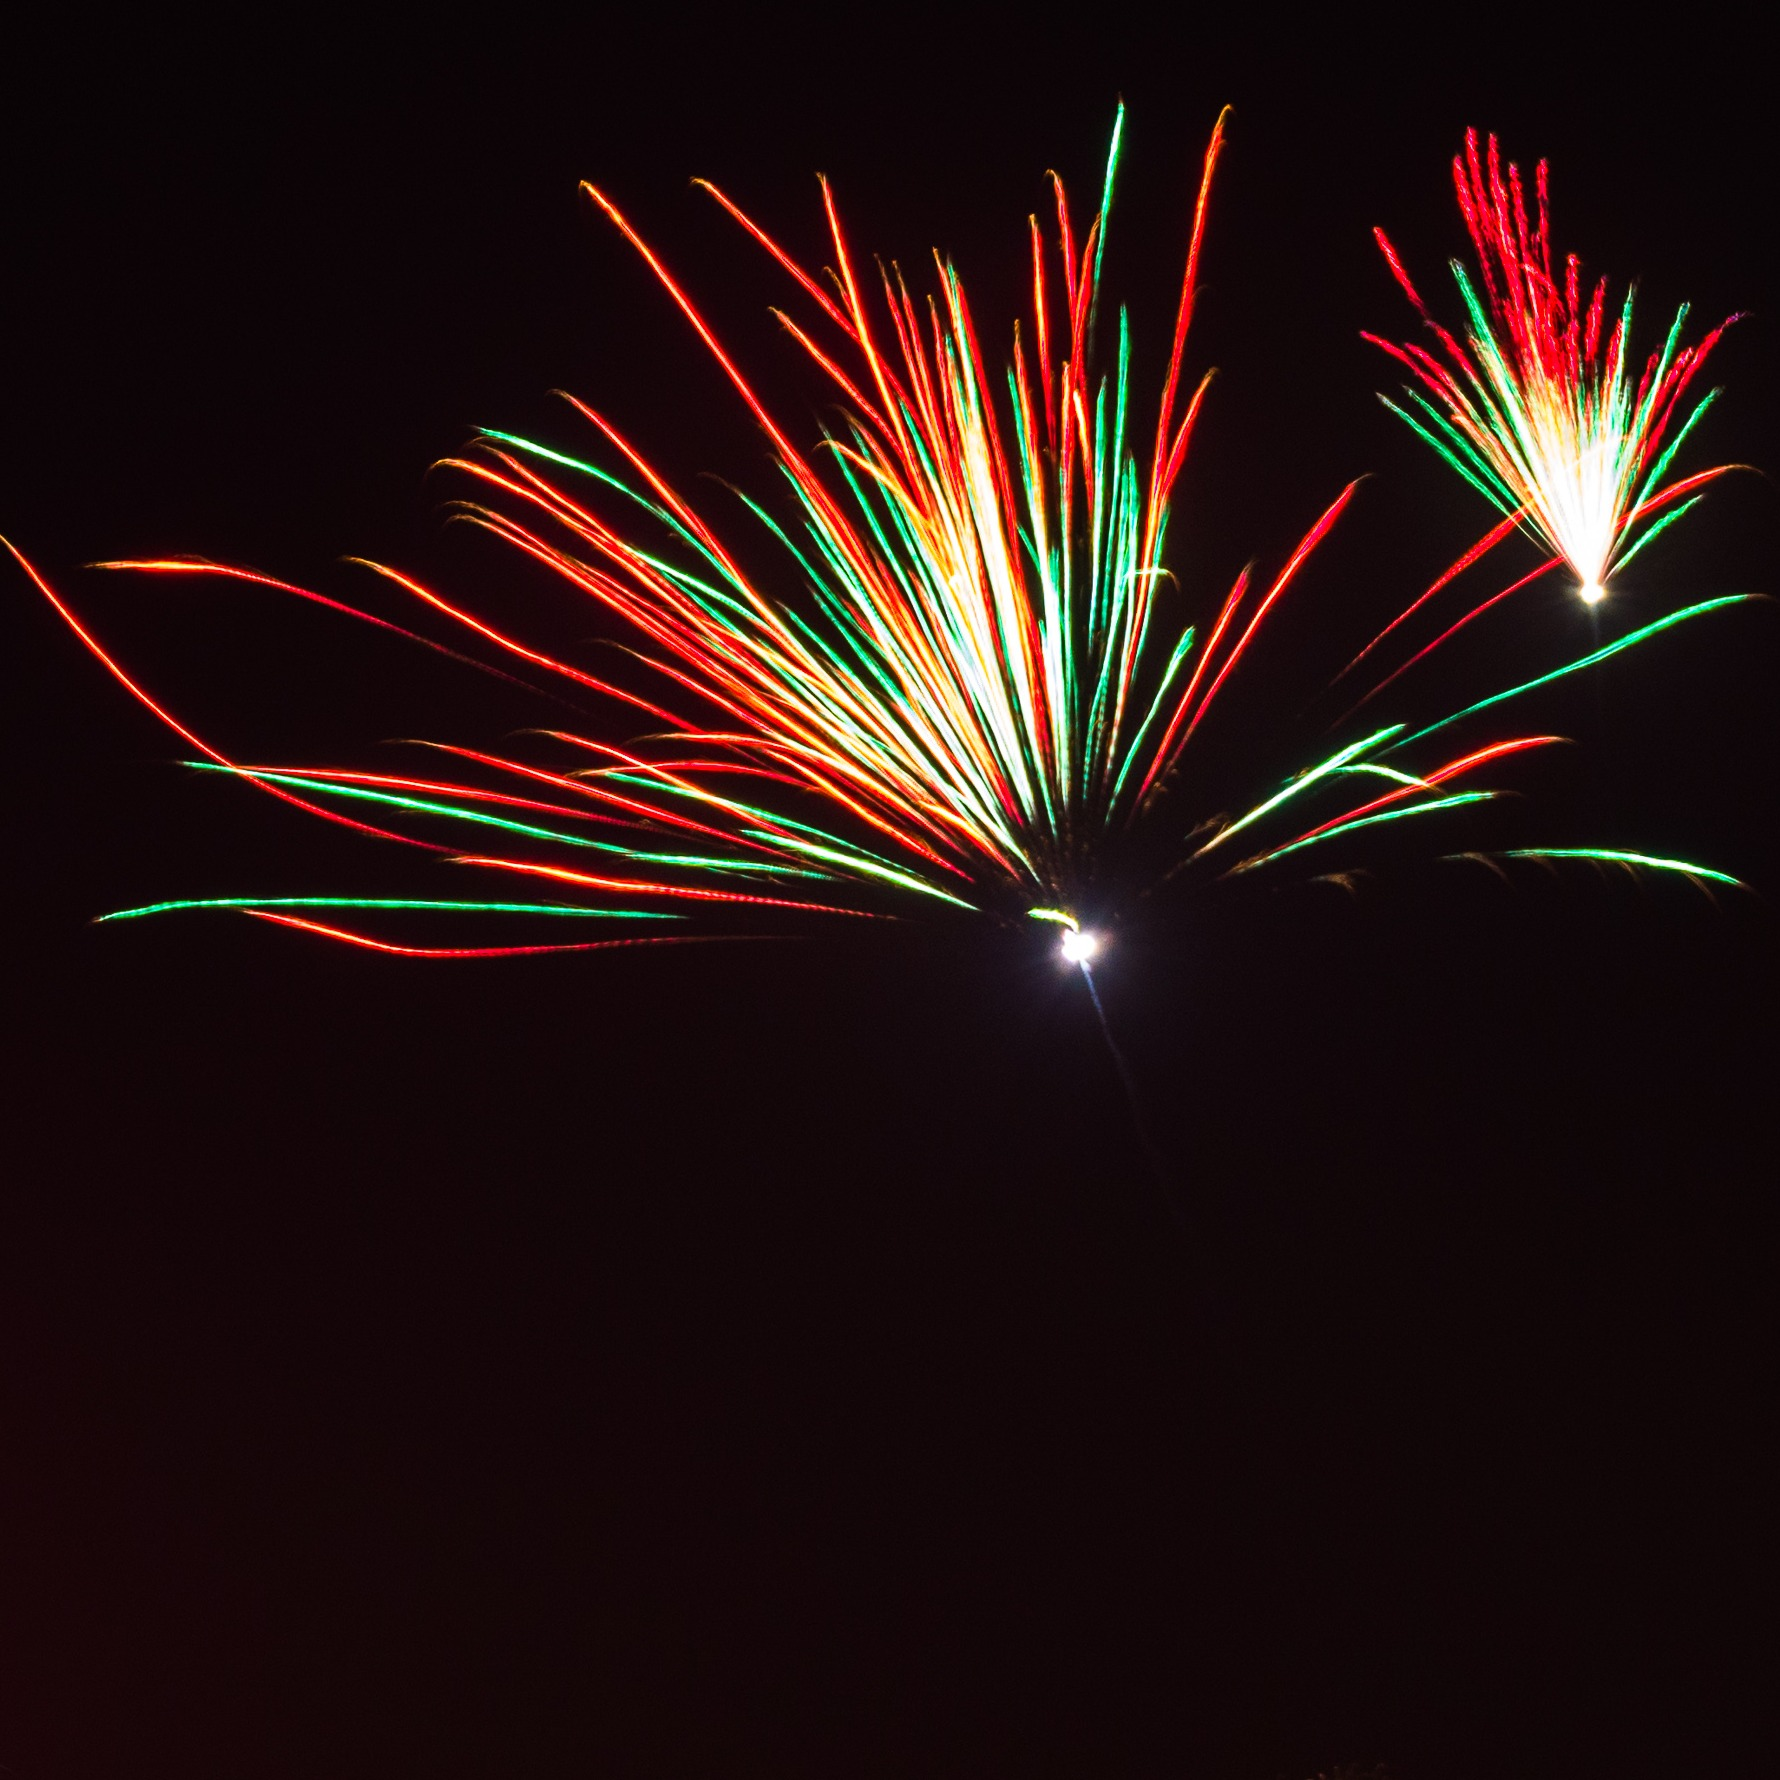
\includegraphics[width=\linewidth]{images/feuerwerk.jpg}\\
    \end{column}%
    \hfill%
    \begin{column}{0.495\textwidth}%
      \only<1>{\includegraphics[width=\linewidth]{build/plots/fireworks_deuter_50.jpg}}%
      \only<2>{\includegraphics[width=\linewidth]{build/plots/fireworks_deuter_100.jpg}}%
    \end{column}%
  \end{columns}%

  \begin{center}%
    \only<1>{Moderate Deuteranomalie}%
    \only<2>{Deuteranopie}%
  \end{center}%
\end{frame}


\section{15 Minuten Einführung in Farbtheorie}

\section{Datenvisualisierung}
\bumper{Datenvisualisierung}

\begin{frame}[t]{Warum?}
  \begin{tikzpicture}[remember picture, overlay, shift=(current page.center)]
    \node[anchor=north west, fill=black, text=green!70!white] (A) at (-0.5\textwidth, 0.4\textheight) {
      \tiny\input{build/img.tex}%
    };
    \node[anchor=south east, visible on=<2->] (B) at (0.5\textwidth, -0.5\textheight) {{
      \includegraphics[height=4cm]{build/plots/u_sw.png}
    }};
    \draw[line width=5pt, ->, visible on=<2->] (A.south) to [out=270, in=180] (B.west);
    \node [xshift=1cm, yshift=-1.5cm] at (A.south) {\Large colormap}; 
  \end{tikzpicture}%
\end{frame}

\begin{frame}[t]{Wahl der Farbskala hat Konsequenzen}
  \begin{center}
    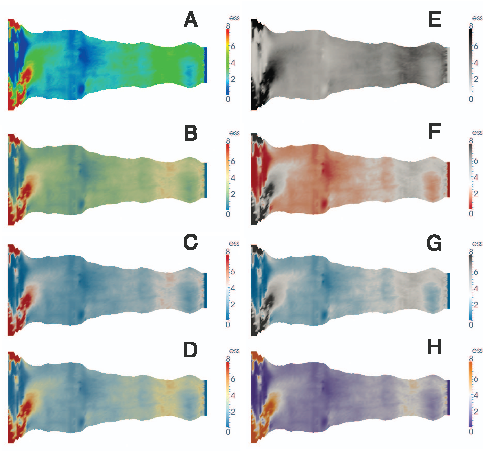
\includegraphics[height=0.7\textheight]{images/heartdisease.pdf}
  \end{center}

  \leavevmode
  \foreignblockquote{english}{%
    We show statistically significant results demonstrating [...]
    that a perceptually appropriate color map
    leads to \textbf{fewer diagnostic mistakes} than a rainbow color map.%
  }\\[0.5\baselineskip]
  \small\cite{heartdisease}
\end{frame}


\begin{frame}[t]{Wahl der Farbskala hat Konsequenzen}  
  \centering

  \includegraphics[height=0.7\textheight]{build/plots/norainbow.pdf}

  \begin{tcolorbox}[colframe=black, colback=white, fontupper=\raggedright\bfseries\zigarette, width=0.68\textwidth, boxrule=4pt, sharp corners]
    Benutzung der Rainbow-Colormap fügt Ihnen
    und den Menschen in Ihrer Umgebung erheblichen Schaden zu.
  \end{tcolorbox}
\end{frame}


\end{document}
